\section{章节标题示例:技术概述}

\subsection{技术定义与特性}

% 请在此处填写您研究的技术定义与其主要特性说明。
% 示例:
% 本节应简要介绍所研究技术的基本概念、定义、原理以及主要特点,适合引用权威文献支持。

\begin{figure}[htbp]
    \centering
    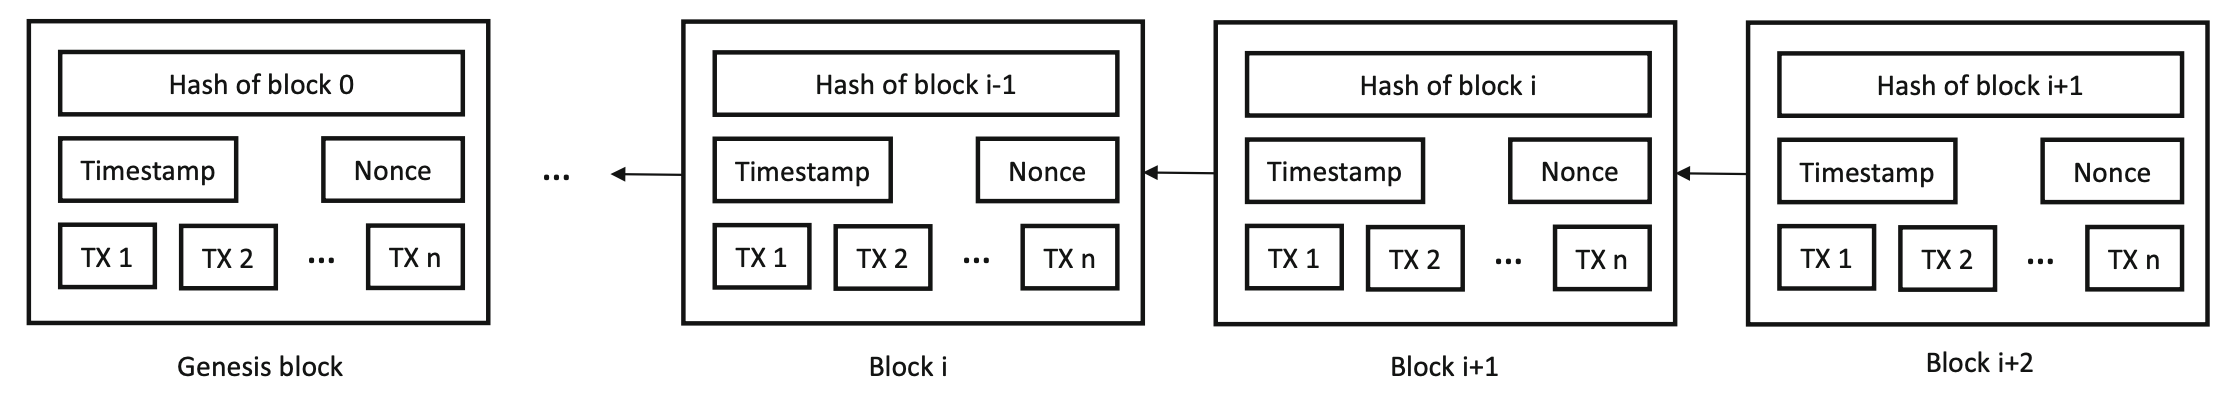
\includegraphics[width=\textwidth]{Imgs/BlockChain.png}
    \caption{示意图示例:此处填写图片说明文字}
    \label{fig:example_structure}
\end{figure}

% 插图说明:
% 使用 \includegraphics 插入图片,推荐图片存放在项目文件夹中的 Imgs 目录下。
% 使用 \caption{} 添加图标题,使用 \label{} 方便文中引用。

\subsection{工作原理}

% 请在此处描述所研究技术的基本工作机制或整体流程。
% 可以使用如下格式描述流程:
% (1)步骤一描述……
% (2)步骤二描述……
% (3)步骤三描述……

% 示例无序列表:
\begin{itemize}
    \item 特性一:请填写特性描述。
    \item 特性二:请填写特性描述。
    \item 特性三:请填写特性描述。
\end{itemize}

% 插入参考文献示例:
% 文中引用示例:\cite{sample2024}
% 请在参考文献文件 reference.bib 中添加相关条目。